\chapter{Approach}\label{chap:approach}

As stated in Section \ref{sec:goals}, the main objective of this thesis is to bring the Oghma framework to a web environment. This section describes the work plan for the project that will serve as the basis for the dissertation writing.


\section{Work Plan}\label{sec:work_plan}

The planning shown on Fig. \ref{fig:work_plan} was created based on the priorities of the tasks as well precedences between them. An initial study will be made regarding the Oghma framework, adaptive object-models architectures and the underlying design patterns that allow them to work, with an expected duration of four weeks. During that initial investigation, research will be performed regarding the best GUI patterns that allow end-users to modify the domain model for the application, with an expected duration of four weeks, bringing the total time research and investigation to six weeks. During the final stages of initial research, the knowledge acquired is sufficient to start the development of the project which will serve as the basis for the dissertation report. The last phase of implementation will be coupled with tests and validation by external parties.

\begin{figure}[H]
  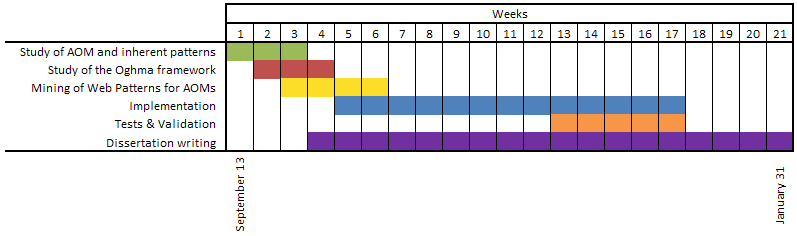
\includegraphics[width=170mm]{work_plan_small.png}
  \caption{Work plan for the duration of the thesis}
  \label{fig:work_plan}
\end{figure}

